% !TEX encoding = UTF-8 Unicode
\documentclass[11pt, a4paper, oneside]{article}
\usepackage[onehalfspacing]{setspace}		% One half spacing
\usepackage{hyperref}					% Hyperlinks on pdf (Should be called before Geometry)
\usepackage[a4paper, 					% Page Layout
                     %showframe,				% This shows the frame
                     twoside, includehead,
                     footskip=7mm, headsep=6mm, headheight=4.8mm,
                     marginparsep=2mm, marginparwidth=22mm,
                     top=25mm, bottom=25mm, inner=30mm, outer=25mm]{geometry}
\usepackage{sansmathfonts}				% Sans Serif equations
\usepackage[T1]{fontenc}					% Output font encoding for international characters
\usepackage[utf8]{inputenc}				% Encoding of files: utf8
\renewcommand*\familydefault{\sfdefault} 		% Sans Serif as default font
%
\usepackage[spanish, es-tabla, es-nodecimaldot]{babel}
\addto\captionsspanish{\renewcommand{\contentsname}{Contenido}}
%
\usepackage[table]{xcolor}
\usepackage{graphicx}
\usepackage{pdfpages}
\usepackage{array}
\hypersetup{
    colorlinks=true,
    linkcolor=blue,
    filecolor=magenta,      
    urlcolor=blue,
}
\urlstyle{same}
\usepackage{tikz}
\RequirePackage{caption} 				% Caption customization
\captionsetup{justification=centerlast,font=small,labelfont=sc,margin=1cm}

\usepackage{array}
\newcommand{\PreserveBackslash}[1]{\let\temp=\\#1\let\\=\temp}
\newcolumntype{C}[1]{>{\PreserveBackslash\centering}p{#1}}
\newcolumntype{R}[1]{>{\PreserveBackslash\raggedleft}p{#1}}
\newcolumntype{L}[1]{>{\PreserveBackslash\raggedright}p{#1}}

\begin{document}
\begin{titlepage}
	\onehalfspacing
	\enlargethispage{0.65\baselineskip}
	\begin{tikzpicture}[remember picture, overlay]
		\coordinate (top_right) at 
		    ([xshift=-2.5cm, yshift=-2.5cm]current page.north east);
		\coordinate (top_left) at 
		    ([xshift=2.3cm, yshift=-1.8cm]current page.north west);
		\coordinate (bottom_right) at 
		    ([xshift=-1.8cm, yshift=1.8cm]current page.south east);
		\node[inner sep=0, anchor=north east] at (top_right) {\href{http://www.itba.edu.ar}{
\includegraphics[height=19mm, trim={180 200 200 200}, clip]{figs/logo_itba.png}}};
		\draw[double, line width = 0.5pt] (top_left) rectangle (bottom_right);
	\end{tikzpicture}
	\par
	\vspace{-0.8cm}
	\noindent \textbf{CENTRO DE INVESTIGACIÓN Y DESARROLLO EN}\par
	\noindent \textbf{ELECTRONICA INDUSTRIAL (CIDEI)}\par
	\vspace{3cm}
	\begin{center}
		{\Huge \textbf{Plataforma ARiCE}\par}
		{\huge \textbf{Primeros Pasos Apio}\par}
	\end{center}
	\vspace{1cm}
	\begin{center}
		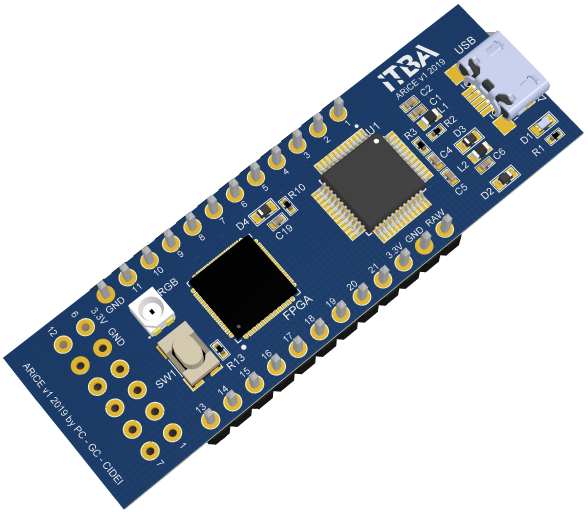
\includegraphics[width=8cm]{figs/fig1a.png}
	\end{center}
	\vfill
	\noindent \textbf{AUTORES:} Dr. Ing. Pablo \textsc{Cossutta} - Ing. Gonzalo \textsc{Castelli} - Rodrigo \textsc{Devesa} \par
	\vfill
	\begin{center}
		\textbf{CIUDAD AUTÓNOMA DE BUENOS AIRES}\\
		\textbf{2018-2019}\par
	\end{center}
\end{titlepage}

\tableofcontents
\newpage

\section{Introducción}
Este proyecto es una plataforma de código abierto, la cual se muestra en la Fig. \ref{fig1}, basado en una placa FPGA de bajo costo y bajo consumo de \href{http://www.latticesemi.com}{Lattice Semiconductor}. Tiene como objetivo ser utilizada en una amplia gama de aplicaciones de procesamiento de señales y control, tanto para la educación como para la industria.
%
\begin{figure}[h!]
	\centering
	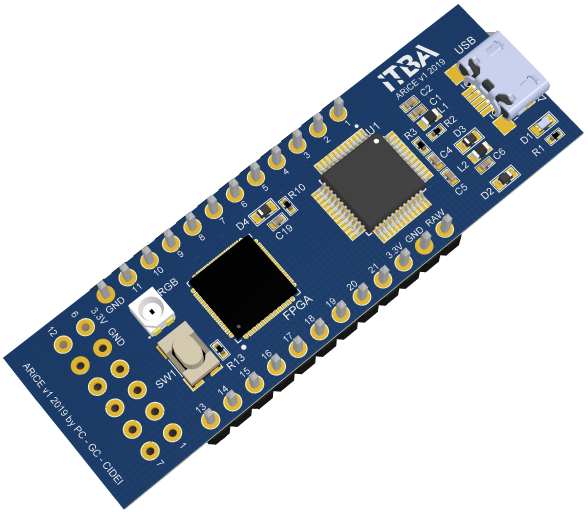
\includegraphics[width=8cm]{figs/fig1a.png}\\
	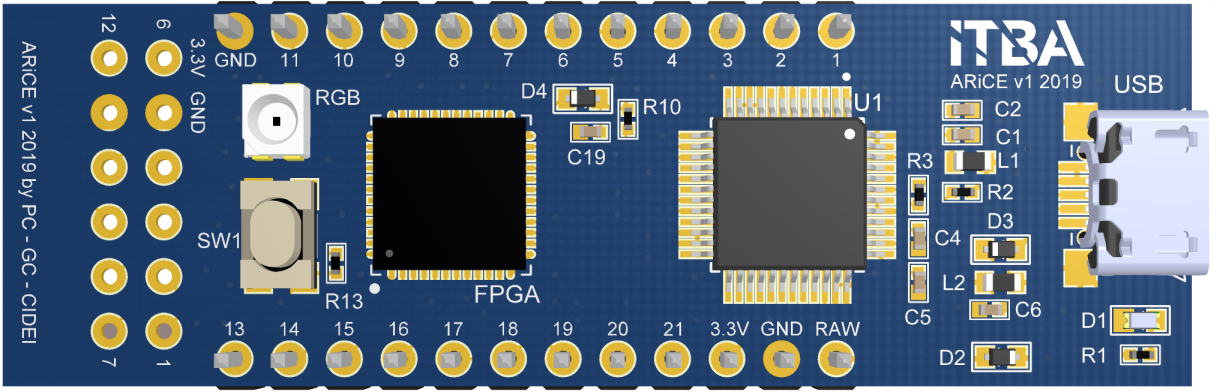
\includegraphics[width=6cm]{figs/fig1b.png}%
	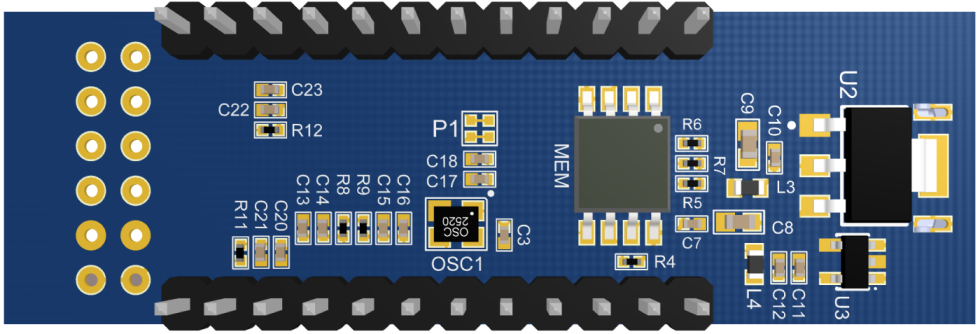
\includegraphics[width=6cm]{figs/fig1c.png}
	\caption{Vistas de la placa}
	\label{fig1}
\end{figure}

%\subsection{Project file sources}
%The following list shows the different file sources for this project:
%\begin{itemize}
%	\item Getting Started Guide and Documentation: \href{https://github.com/pcossutta/Lattice-FPGA/tree/master/Documents/Manuals}{GitHub manuals}
%	\item PCB and Schematics: \href{https://workspace.circuitmaker.com/Projects/Details/Gonzalo-Castelli/FPGA-ITBA}{Circuit Maker} and \href{https://github.com/pcossutta/Lattice-FPGA/tree/master/Altium}{GitHub Altium Project Files}
%	\item \href{https://github.com/pcossutta/Lattice-FPGA/tree/master/Examples/LedExample}{Example code} for the Lattice Radiant software.
%\end{itemize}

\section{Primeros pasos}
Para comenzar a utiliza la plataforma hay que cumplir tres pasos. El primero es descargar e instalar el software, después crear un proyecto incluyendo los archivos de código necesarios y por último cargar el programa en la memoria interna del FPGA usando un cable USB.

\subsection{Descargando el software}
Antes de usar la placa, es necesario descargar el software para programar la FPGA Lattice iCE40-UP5K. En este tutorial se va a utilizar la distribución basada en \href{https://apiodoc.readthedocs.io/en/stable/index.html}{Apio Open Source Ecosystem for FPGAs}, la cual permite sintetizar, implementar y verificar el código y también programar la FPGA mediante un puerto USB. \href{https://apiodoc.readthedocs.io/en/stable/index.html}{Python 3.7+} debe ser instalado previamente para poder instalar Apio.

Durante la instalación de Python debe asegurarse de seleccionar "\textbf{Customize Installation}". Luego, dentro de las opciones adicionales, seleccionar la instalación de \textit{pip},como se muestra en la Fig. \ref{fig2}, dado que se necesita para descargar e instalar el paquete de Apio.

\begin{figure}[h!]
    \centering
    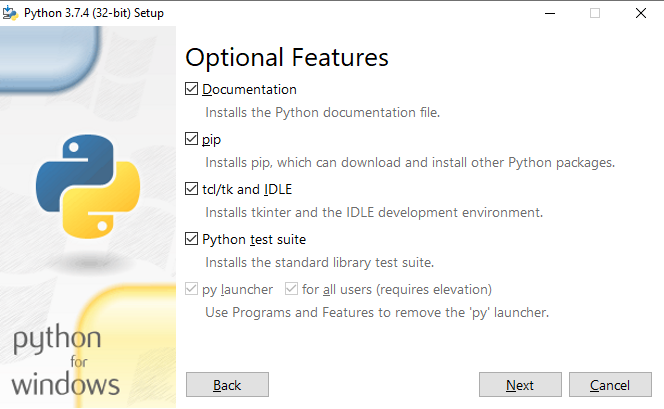
\includegraphics[width=0.8\textwidth]{figs/python_install.png}
    \caption{Configuración de la instalación de Python}
    \label{fig2}
\end{figure}

Una vez finalizada la instalación de Python con pip, se procede a instalar Apio. En Windows, se debe abrir una consola de comandos e ingresar:
\begin{center}
	\texttt{pip install -U apio}
\end{center}
Cuando finaliza, es necesario instalar los paquetes adicionales de Apio utilizando el siguiente comando:
\begin{center}
	\texttt{apio install -{}-all}
\end{center}
Esta proceso puede demorar varios minutos.

\subsection{Creando un nuevo proyecto}
Una vez instalado el software, el siguiente paso es crear una nueva carpeta para el proyecto, y empezar as escribir el código. Un ejemplo de proyecto que utiliza el LED RGB montado en la placa esta disponible en nuestro repositorio Github. Después de descargar los archivos, se colocan en una carpeta fácilmente accesible desde donde ejecutaremos el código.

Use el comando \texttt{cd} seguido por la dirección de la carpeta de proyecto para seleccionarla y trabajar sobre ella. Por ejemplo, si el proyecto esta en una carpeta llamada "fpga\_project" en el Escritorio, use:
\begin{center}
	\texttt{cd Desktop/fpga\_project}
\end{center}

Una vez seleccionada la carpeta a utilizar, generamos el archivo de configuración .init adecuado para nuestra placa, ya que Apio soporta varias plataformas de FPGA diferentes. Para hacer esto, use el comando:
\begin{center}
	\texttt{apio init -{}-board upduino2}
\end{center}

Ahora puede usar el comando:
\begin{center}
	\texttt{apio build}
\end{center}
 para asegurar que el proyecto esta correctamente configurado. La carpeta debería contener al menos 3 archivos; un .v con el código del programa, un .pcf con información de entradas y salidas para el programa, y el archivo .init que acabamos de crear. Si el programa compila correctamente, puede pasar a programar la placa FPGA.
 
\subsection{Programando la placa}
Ahora que el proyecto esta armado, podemos cargar el programa a nuestra placa para ejecutarlo.

Conecte la FPGA a la PC con un cable USB, espere unos segundos para que Windows configure los controladores, y luego utilice el siguiente comando para programar la placa:
\begin{center}
	\texttt{apio upload}
\end{center}

El proceso puede demorar algunos segundos. Si todo funcionó correctamente, la placa debería configurarse desde la memoria flash interna y el LED comenzará a prenderse y a cambiar de color.

\subsection{Simulando el diseño}
Para simular el diseño ejecutar el siguiente comando:
\begin{center}
	\texttt{apio sim}
\end{center}

Se cargará el visualizador \href{http://gtkwave.sourceforge.net}{GTKWave} y se podrá analizar el resultado de la simulación.

% !TEX encoding = UTF-8 Unicode
\newpage
\section{Información de las conexiones}
La placa posee múltiples pines de E/S, junto con alimentaciones, distribuidas en los conectores laterales y frontales del circuito impreso. La siguiente lista provee una breve descripción de estas señales:
\begin{itemize}
	\item IOT\_XX corresponde a pines estándar de E/S. En el modo usuario, después de la configuración, estos pines pueden ser utilizados como E/S según el usuario y corresponden al banco superior (top, donde xx = ubicación de E/S)
	\item IOB\_XX corresponde a pines estándar de E/S. En el modo usuario, después de la configuración, estos pines pueden ser utilizados como E/S según el usuario y corresponden al banco inferior (bottom, donde xx = ubicación de E/S
	\item RAW VCC. La alimentación de la placa cuando utiliza una fuente de alimentación externa. La alimentación puede provenir tanto del conector USB como del pin RAW VCC (Tensión mínima de 4.5V y máxima de 6V)
	\item 3.3V. Salida de 3.3V generada por el regulador de tensión lineal interno. No excede los 500mA
	\item GND. Pines de referencia
	\item Las señales que contienen los sufijos G1, G3 y G6 pueden ser utilizadas tamos como pines estándar de E/S o señales globales con gran cantidad de conexiones internas o cómo líneas de clock o reset. Estos pines se encuentran conectados a los buffers globales GBUF1, GBUF3 y GBUF6 respectivamente.
\end{itemize}

\newpage
La Tabla \ref{table1} muestra la correspondencia entre la asignación de pines, el nombre de las señales y el pad correspondiente al encapsulado de la FPGA.
\definecolor{myHdr}{rgb}{0.81000,0.8800,0.9400}%
\begin{table}[h!]
	\renewcommand{\arraystretch}{1.3}
	\caption{Conexiones}
	\label{table1}
	\begin{tabular}[t]{C{0.12\textwidth} C{0.12\textwidth} C{0.15\textwidth}}
		\bfseries Pin Placa & \bfseries Pin FPGA & \bfseries Señal \\ \hline
		\rowcolor{myHdr} \multicolumn{3}{c}{\bfseries Conexiones Laterales} \\ \hline
		1 & 20 & IOB 25B G3 \\
		2 & 21 & IOB 23B \\
		3 & 23 & IOT 37A \\
		4 & 25 & IOT 36B \\
		5 & 26 & IOT 39A \\
		6 & 27 & IOT 38B \\
		7 & 31 & IOT 42B \\
		8 & 32 & IOT 43A \\
		9 & 34 & IOT 44B \\
		10 & 36 & IOT 48B \\
		11 & 37 & IOT 45A G1 \\
		12 & - & GND \\
		& & \\
		13 & 2 & IOB 6A \\
		14 & 6 & IOB 13B \\
		15 & 9 & IOB 16A \\
		16 & 10 & IOB 18A \\
		17 & 11 & IOB 20A \\
		18 & 12 & IOB 22A \\
		19 & 13 & IOB 24A \\
		20 & 18 & IOB 31B \\
		21 & 19 & IOB 29B \\
		22 & - & 3.3V \\
		23 & - & GND \\
		24 & - & RAW VCC \\
	\end{tabular}
	\quad
	\begin{tabular}[t]{C{0.12\textwidth} C{0.12\textwidth} C{0.15\textwidth}}
		\bfseries Pin Placa & \bfseries Pin FPGA & \bfseries Señal \\ \hline
		\rowcolor{myHdr} \multicolumn{3}{c}{\bfseries Conexiones Frontales} \\ \hline
		1 & 4 & IOB 8A \\
		2 & 3 & IOB 9B \\
		3 & 47 & IOB 2A \\
		4 & 44 & IOB 3B G6 \\
		5 & - & GND \\
		6 & - & 3.3V \\
		7 & 48 & IOB 4A \\
		8 & 45 & IOB 5B \\
		9 & 38 & IOT 50B \\
		10 & 42 & IOT 51A \\
		11 & - & GND \\
		12 & - & 3.3V \\
		& & \\
		\bfseries Pin Placa & \bfseries Pin FPGA & \bfseries Señal \\ \hline
		\rowcolor{myHdr} \multicolumn{3}{c}{\bfseries No Conectados} \\ \hline
		 - & 43 & IOT 49A \\
		- & 46 & IOB 0A \\
		- & 28 & IOT 41A \\	
		& & \\
		& & \\
		\bfseries Color LED & \bfseries Pin FPGA & \bfseries Señal \\ \hline
		\rowcolor{myHdr} \multicolumn{3}{c}{\bfseries LED RGB interno} \\   \hline
		Azul & 39 & RGB0 \\
		Verde & 40 & RGB1 \\
		Rojo & 41 & RGB2 \\
	\end{tabular}
\end{table}

\newpage
Los pares diferenciales se muestran en la Tabla \ref{table2}. Los mismos están agrupados y en colores, dónde fondo blanco corresponde al terminal positivo y celeste al negativo.
%
\begin{table}[h!]
	\renewcommand{\arraystretch}{1.3}
	\caption{Pares Diferenciales}
	\vspace{0.5em}
	\label{table2}
	\centering
	\begin{tabular}{C{0.12\textwidth} C{0.12\textwidth} C{0.15\textwidth}}
		\bfseries Pin Placa & \bfseries Pin FPGA & \bfseries Señal \\ \hline
		\rowcolor{myHdr}  3 & 23 & IOT 37A \\
		4 & 25 & IOT 36B \\ \hline
		\rowcolor{myHdr}  5 & 26 & IOT 39A \\
		6 & 27 & IOT 38B \\ \hline
		\rowcolor{myHdr}  8 & 32 & IOT 43A \\
		7 & 31 & IOT 42B \\ \hline
		\rowcolor{myHdr}  11 & 37 & IOT 45A G1 \\
		9 & 34 & IOT 44B \\ \hline
		\rowcolor{myHdr}  2 & 21 & IOB 23B \\
		18 & 12 & IOB 22A \\ \hline
		\rowcolor{myHdr}  2 & 3 & IOB 9B \\
		1 & 4 & IOB 8A \\ \hline
		\rowcolor{myHdr}  4 & 44 & IOB 3B G6 \\
		3 & 47 & IOB 2A \\ \hline
		\rowcolor{myHdr}  8 & 45 & IOB 5B \\ 
		7 & 48 & IOB 4A \\ \hline
		\rowcolor{myHdr}  10 & 42 & IOT 51A \\ 
		9 & 38 & IOT 50B \\
	\end{tabular}
\end{table}

\section{Circuito Impreso Libre}
los archivos de diseño, diagramas esquemáticos y el listado de componentes se encuentran disponibles en el repositorio de GitHub. Los archivos del proyecto realizado en Altium y los Gerbers de fabricación están disponibles. Además el diseño está publicado utilizando herramientas libres como \href{https://workspace.circuitmaker.com/}{Circuit Maker} y \href{http://www.kicad-pcb.org}{KiCad}.

\newpage
\subsection{Listado de componentes}
En la Tabla \ref{table3} se incluye todos los componentes de la plataforma ARiCE. Para mayor información se incluye el link con la mayoría de las hojas de datos de los componentes utilizados.
%
\begin{table}[h]
	\renewcommand{\arraystretch}{1.3}
	\caption{Listado de componentes}
	\vspace{0.5em}
	\label{table3}
	\centering
	\begin{tabular}{p{4cm} C{0.5cm} c C{1cm} p{2cm}}
		\bfseries Nombre & \bfseries Cant. & \bfseries Código del Fabricante & \bfseries Valor & \bfseries Footprint \\ \hline
		C2, C3, C4, C5, C6, C10, C12, C14, C16, C18, C19, C21, C23 & 13 & \href{http://www.samsungsem.com/kr/support/product-search/mlcc/CL05B104KA5NNNC.jsp}{CL05B104KA5NNNC} & 0.1uF & 0402 \\ \hline
		C8, C9 & 2 & \href{http://www.yageo.com/documents/recent/UPY-GPHC_X5R_4V-to-50V_25.pdf}{CC0603KRX5R8BB105} & 1uF & 0603 \\ \hline
		C1, C7, C11, C13, C15, C17, C20, C22 & 8 & \href{https://product.tdk.com/info/en/catalog/datasheets/mlcc_commercial_lowprofile_en.pdf}{CGB2A1JB1E105M033BC} & 1uF & 0402 \\ \hline
		R1 & 1 & \href{http://www.yageo.com/documents/recent/PYu-RC_Group_51_RoHS_L_9.pdf}{RC0402JR-071KL} & 1K$\Omega$ & 0402 \\ \hline
		R2 & 1x& \href{http://www.yageo.com/documents/recent/PYu-RC_Group_51_RoHS_L_9.pdf}{RC0402FR-072K2L} & 2.2k$\Omega$ & 0402 \\ \hline
		R3, R4, R5, R6, R7, R13 & 6 & \href{http://www.yageo.com/NewPortal/yageodocoutput?fileName=/pdf/R-Chip/PYu-RC_51_RoHS_P_0.pdf}{RC0402JR-0710KP} & 10k$\Omega$ & 0402 \\ \hline
		R8, R9, R10, R11, R12 & 5 & \href{http://www.yageo.com/NewPortal/yageodocoutput?fileName=/pdf/R-Chip/PYu-AC_51_RoHS_L_6.pdf}{AC0402JR-071RL} & 1$\Omega$ & 0402 \\ \hline
		L1 & 1 & \href{http://assets.lairdtech.com/home/brandworld/files/HI0603P600R-10.pdf}{HI0603P600R-10} & 10mH & 0603 \\ \hline
		L2, L3, L4 & 3 & \href{https://www.murata.com/en-us/products/productdata/8796741599262/ENFA0004.pdf}{BLM18HE601SN1D} & 10mH & 0603 \\ \hline
		RGB & 1 & \href{https://www.cree.com/led-components/media/documents/1273-CLMVC-FKA.pdf}{CLMVC-FKA-CL1D1L71BB7C3C3} & & 4-PLCC \\ \hline
		D1 & 1 & \href{http://optoelectronics.liteon.com/upload/download/DS-22-99-0224/LTST-C190TBKT.PDF}{LTST-C190TBKT} & & 0603 \\ \hline
		U1 & 1 & \href{http://www.ftdichip.com/Support/Documents/DataSheets/ICs/DS_FT232H.pdf}{FT232HL-REEL} & & 48-LQFP (7x7) \\ \hline    
		U2 & 1 & \href{http://www.ti.com/lit/ds/symlink/tlv1117lv.pdf}{TLV1117LV33DCYR} & & SOT-223-4 \\ \hline
		U3 & 1 & \href{http://www.ti.com/lit/ds/symlink/lp5907.pdf}{LP5907MFX-1.2/NOPB} & & SOT-23-5 \\ \hline
		OSC1 & 1 & \href{https://media.digikey.com/pdf/Data\%20Sheets/SiTime\%20PDFs/SIT1602A.pdf}{SIT1602AC-73-33S-12.000000G} & & 2.0X1-6MM \\ \hline
		FPGA & 1 & \href{http://www.latticesemi.com/view_document?document_id=51968}{ICE40UP5K-SG48ITR50} & & 48-QFN-7X7 \\ \hline
		USB & 1 & \href{http://www.amphenol-icc.com/media/wysiwyg/files/drawing/10118193.pdf}{10118193-0001LF} & & Micro USB B SMD \\ \hline
		MEM & 1 & \href{https://www.winbond.com/resource-files/w25q32jv%20dtr%20revf%2002242017.pdf}{W25Q32JVSSIQ} & & SOP8 \\ \hline
		D2, D3, D4 & 3 & \href{http://www.comchiptech.com/admin/files/product/CDBU0520-HF-RevA797161.pdf}{CDBU0520} & & 0603/SOD-523F \\ \hline
		SW1 & 1 & \href{https://www.ckswitches.com/media/1465/kxt3.pdf}{PTS810 SJM 250 SMTR LFS} & & SW4-SMD \\
	\end{tabular}
\end{table}

\subsection{Diagramas esquemáticos}
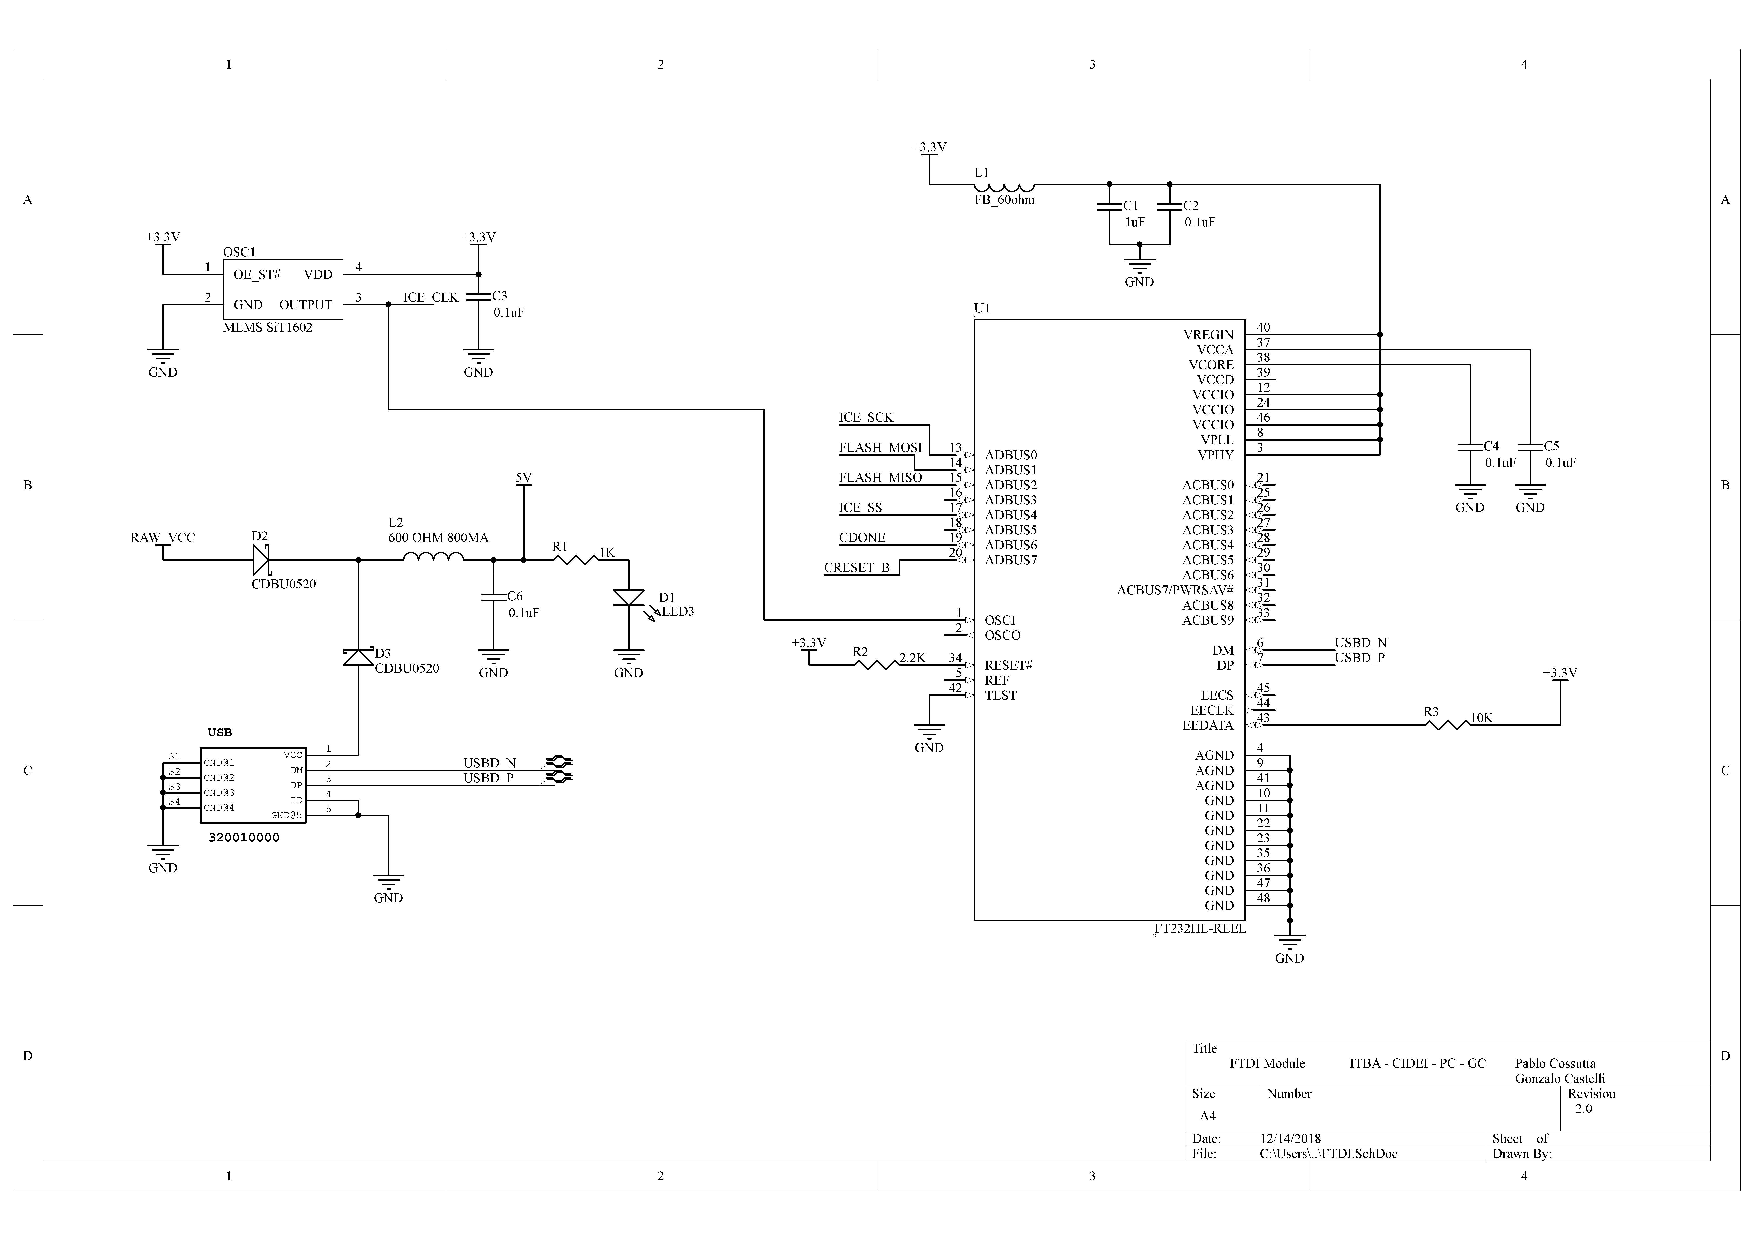
\includepdf[landscape=true]{figs/ftdi.pdf}
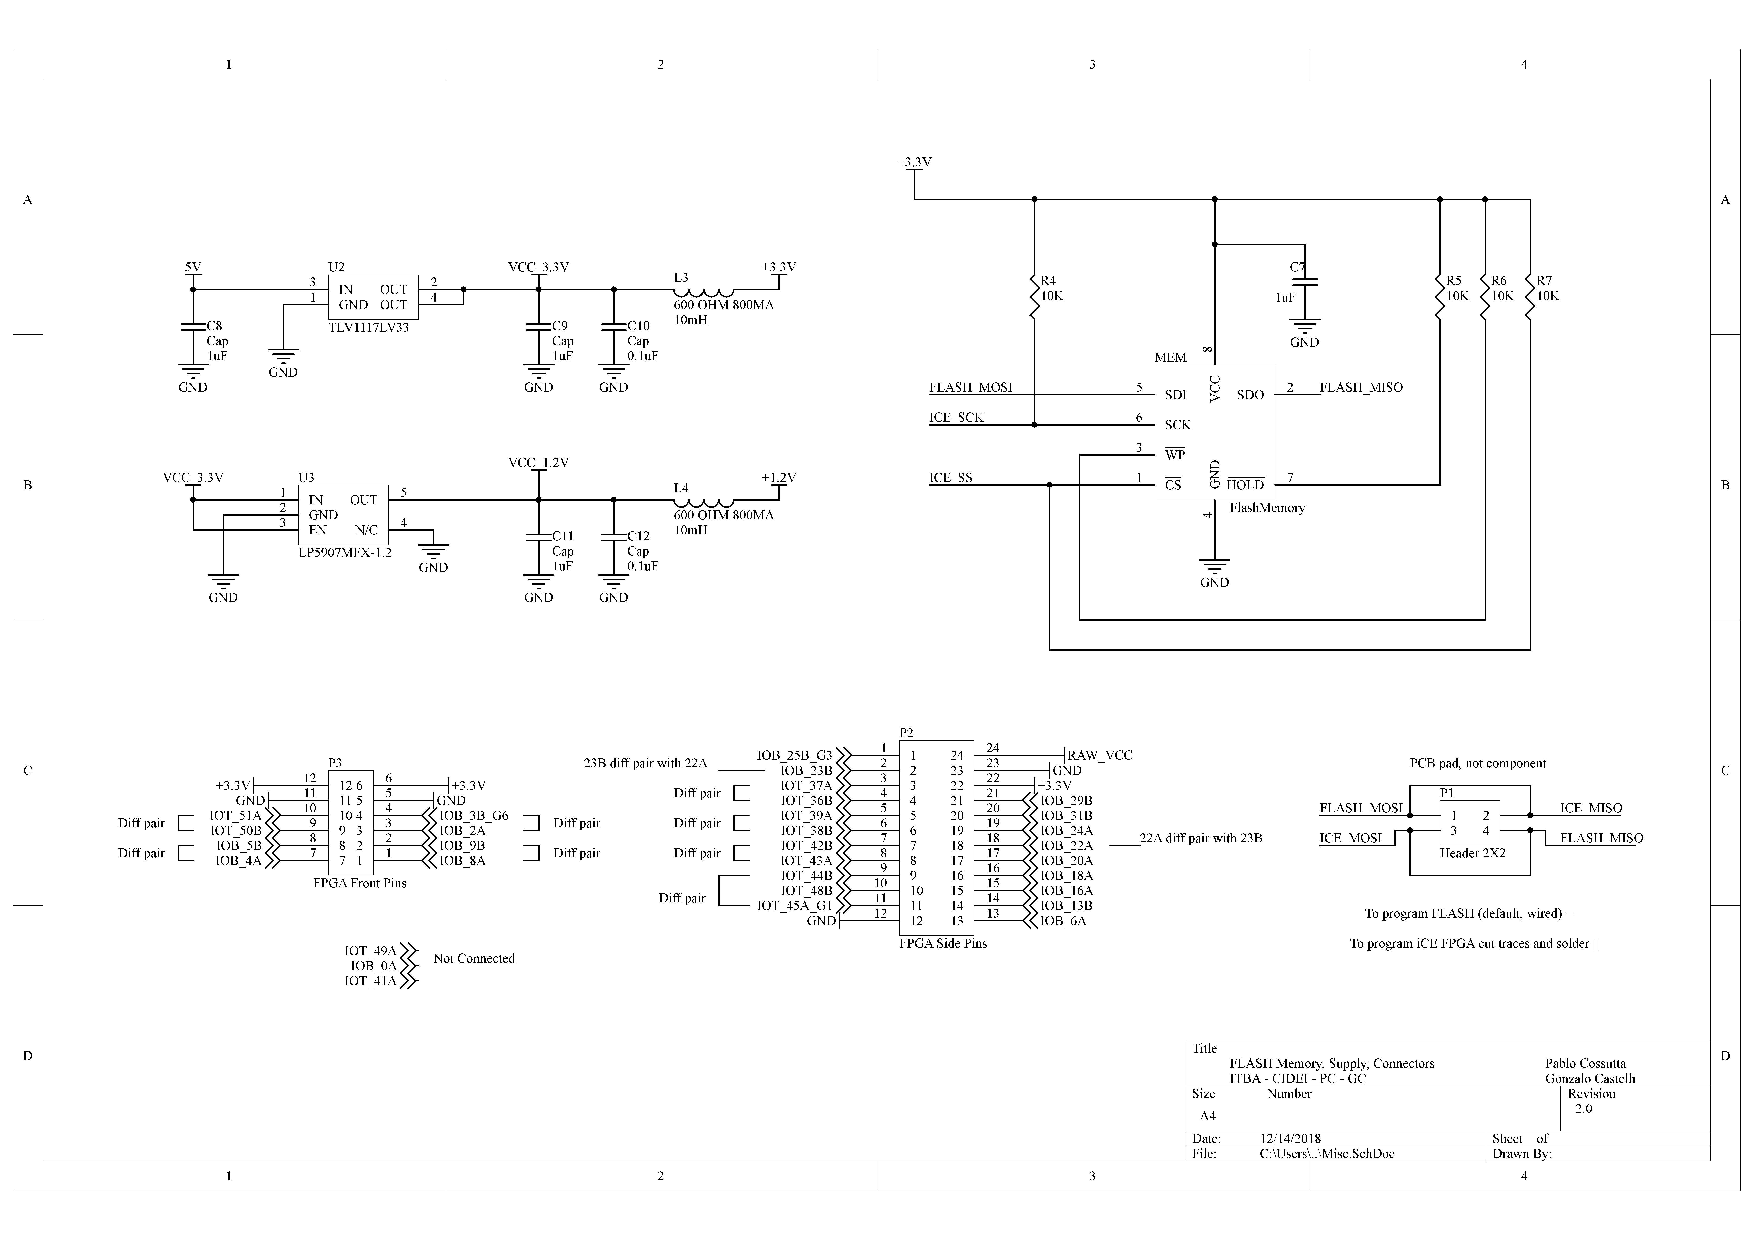
\includepdf[landscape=true]{figs/misc.pdf}
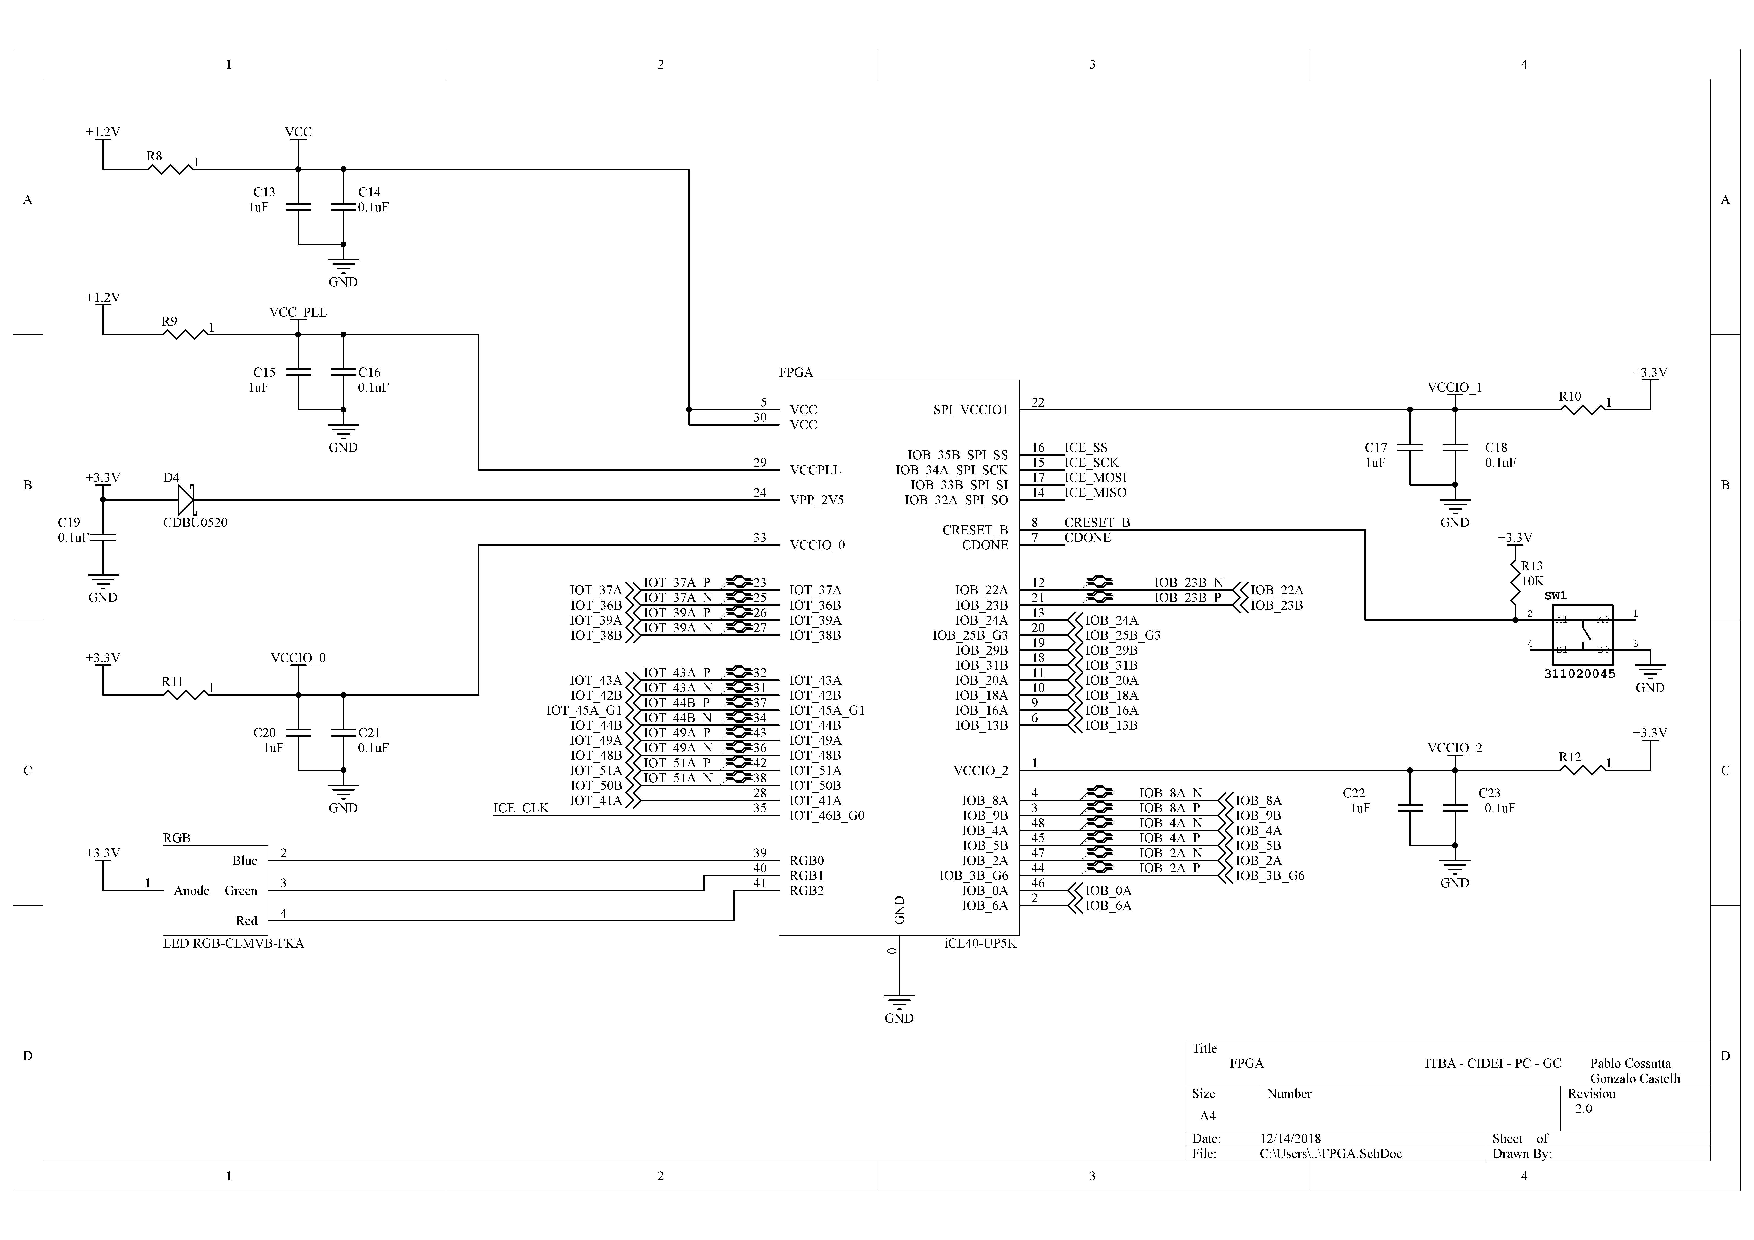
\includepdf[landscape=true]{figs/fpga.pdf}

\section{Licencia}
Este proyecto se provee bajo la licencia \textit{Creative Commons Attribution Share-Alike}, lo que significa que puede ser utilizado libremente, adaptado a sus necesidades, sin necesidad de solicitar o pagar un permiso, siempre y cuando se denote apropiadamente los créditos del creador original y se libere el diseño bajo la misma licencia. Para mayor información visitar el sitio web \href{https://creativecommons.org/licenses/by-sa/3.0/}{Creative Commons}.

\section{Agradecimientos}
Este proyecto se inspira y basa en los manuales oficiales y las herramientas detalladas en \href{http://www.latticesemi.com/en/Products/DevelopmentBoardsAndKits/iCE40UltraPlusBreakoutBoard.aspx}{iCE40 UltraPlus Breakout Board} de Lattice Semiconductors y en la documentación de la FPGA, iCE40UP5K.
\end{document}
